\documentclass[11pt,a4paper]{article}

\usepackage[T1]{fontenc}
\usepackage[utf8]{inputenc}
\usepackage[french]{babel}
\usepackage{lmodern}
\usepackage{geometry}
\usepackage{amsmath}
\usepackage{booktabs}
\usepackage{graphicx}
\usepackage{float}
\usepackage{hyperref}

\geometry{margin=2.4cm}
\graphicspath{{graphs/}{../graphs/}}
\hypersetup{colorlinks=true,linkcolor=blue,urlcolor=blue}

\title{TP n\textsuperscript{o}1 -- Test de primalité\\\large Étude des algorithmes et mesures expérimentales}
\author{}
\date{}

\begin{document}
\maketitle
\tableofcontents
\clearpage

\section{Introduction}

L'objectif de ce travail est d'étudier quatre algorithmes qui déterminent si un entier naturel $N$ est premier. Un nombre premier est un entier supérieur ou égal à 2 qui n'admet aucun diviseur autre que 1 et lui-même. Les algorithmes se distinguent par le nombre de diviseurs qu'ils testent. Nous comparons leur complexité théorique et leurs temps d'exécution sur les douze valeurs prescrites dans le sujet.

Les mesures sont réalisées avec la fonction \texttt{clock()} de la bibliothèque \texttt{time.h}. Pour les algorithmes rapides, chaque test est répété jusqu'à ce que la durée totale chronométrée atteigne au moins 50 millisecondes. Le temps présenté est ensuite divisé par le nombre de répétitions. Le résultat de chaque appel est conservé dans une variable \texttt{volatile} afin d'éviter que le compilateur ne supprime les calculs.

\section{Algorithmes étudiés}

Dans les pseudo-codes ci-dessous, le cas $N<2$ est rejeté. Les bornes correspondent aux tests effectués dans le programme.

\subsection{Algorithme A1 : test naïf jusqu'à $N-1$}

A1 teste tous les diviseurs possibles compris entre 2 et $N-1$. Si aucun ne divise $N$, le nombre est premier.

\begin{verbatim}
fonction A1(N)
    si N < 2, retourner faux
    pour i de 2 à N - 1
        si N mod i = 0, retourner faux
    retourner vrai
\end{verbatim}

\subsection{Algorithme A2 : test jusqu'à $N/2$}

Tout diviseur propre de $N$ est inférieur ou égal à $N/2$. A2 évite donc les tests au-delà de cette borne.

\begin{verbatim}
fonction A2(N)
    si N < 2, retourner faux
    pour i de 2 à floor(N / 2)
        si N mod i = 0, retourner faux
    retourner vrai
\end{verbatim}

\subsection{Algorithme A3 : test jusqu'à $\sqrt{N}$}

Les diviseurs d'un entier apparaissent par paires. Si $N=ab$, au moins l'un des deux facteurs est inférieur ou égal à $\sqrt{N}$. Il suffit donc de tester les diviseurs jusqu'à cette limite. Dans le programme, la condition $i\leq N/i$ est utilisée pour représenter cette borne sans calcul flottant.

\begin{verbatim}
fonction A3(N)
    si N < 2, retourner faux
    pour i de 2 tant que i <= N / i
        si N mod i = 0, retourner faux
    retourner vrai
\end{verbatim}

\subsection{Algorithme A4 : test des diviseurs impairs}

A4 traite séparément le nombre 2, rejette immédiatement les nombres pairs supérieurs à 2, puis teste uniquement les diviseurs impairs jusqu'à $\sqrt{N}$.

\begin{verbatim}
fonction A4(N)
    si N < 2, retourner faux
    si N = 2, retourner vrai
    si N est pair, retourner faux
    pour i impair de 3 tant que i <= N / i
        si N mod i = 0, retourner faux
    retourner vrai
\end{verbatim}

\section{Complexité théorique}

Le pire cas considéré est un nombre premier : l'algorithme ne trouve aucun diviseur et parcourt toute sa plage de recherche.

\begin{table}[H]
\centering
\begin{tabular}{lll}
\toprule
Algorithme & Travail au pire cas & Complexité asymptotique \\
\midrule
A1 & $N-2$ candidats & $\Theta(N)$, donc $O(N)$ \\
A2 & environ $N/2-1$ candidats & $\Theta(N)$, donc $O(N)$ \\
A3 & environ $\sqrt{N}$ candidats & $\Theta(\sqrt{N})$ \\
A4 & environ $\sqrt{N}/2$ diviseurs impairs & $\Theta(\sqrt{N})$ \\
\bottomrule
\end{tabular}
\caption{Ordres de grandeur du nombre d'essais au pire cas.}
\end{table}

Les colonnes théoriques générées pour ce rapport sont des proxys du nombre d'opérations. Elles ne représentent pas des secondes mesurées. A2 conserve une complexité linéaire : sa borne réduit le travail d'un facteur constant, mais ne change pas l'ordre asymptotique. A3 passe d'une croissance linéaire à une croissance en racine carrée, ce qui constitue une amélioration asymptotique. A4 garde le même ordre que A3, mais réduit encore le nombre de tests en sautant les diviseurs pairs.

\section{Vérification des entrées}

Les douze valeurs demandées par le sujet sont données ci-dessous, dans leur ordre d'origine. Les quatre algorithmes concluent que chacune est première. Les mêmes valeurs ont également été vérifiées séparément par un test de divisibilité jusqu'à la racine carrée.

\begin{center}
\begin{tabular}{rrrr}
\toprule
$N$ & $N$ & $N$ & $N$ \\
\midrule
1\,000\,003 & 2\,000\,003 & 4\,000\,037 & 8\,000\,009 \\
16\,000\,057 & 32\,000\,011 & 64\,000\,031 & 128\,000\,003 \\
256\,000\,001 & 512\,000\,009 & 1\,024\,000\,009 & 2\,048\,000\,011 \\
\bottomrule
\end{tabular}
\end{center}

\section{Résultats expérimentaux}

Le tableau présente le temps moyen d'une exécution en secondes. Les mesures ont été produites par \texttt{tp1\_runner}; les tableaux CSV détaillés se trouvent dans le dossier \texttt{results/}.

\begin{table}[H]
\centering
\small
\begin{tabular}{r r r r r c}
\toprule
$N$ & A1 (s) & A2 (s) & A3 (s) & A4 (s) & Premier \\
\midrule
1\,000\,003 & 0.00204690625 & 0.00103382813 & $4.11365\times10^{-6}$ & $2.05325\times10^{-6}$ & Oui \\
2\,000\,003 & 0.004110625 & 0.00209284375 & $5.80420\times10^{-6}$ & $2.89975\times10^{-6}$ & Oui \\
4\,000\,037 & 0.00820975 & 0.0041061875 & $8.19116\times10^{-6}$ & $4.11688\times10^{-6}$ & Oui \\
8\,000\,009 & 0.01637175 & 0.00818475 & $1.16116\times10^{-5}$ & $5.81232\times10^{-6}$ & Oui \\
16\,000\,057 & 0.033039 & 0.0168735 & $1.63784\times10^{-5}$ & $8.22681\times10^{-6}$ & Oui \\
32\,000\,011 & 0.066288 & 0.0327485 & $2.32090\times10^{-5}$ & $1.16881\times10^{-5}$ & Oui \\
64\,000\,031 & 0.135053 & 0.065673 & $3.29048\times10^{-5}$ & $1.63765\times10^{-5}$ & Oui \\
128\,000\,003 & 0.259705 & 0.132941 & $4.63745\times10^{-5}$ & $2.31960\times10^{-5}$ & Oui \\
256\,000\,001 & 0.524776 & 0.263725 & $6.55244\times10^{-5}$ & $3.27910\times10^{-5}$ & Oui \\
512\,000\,009 & 1.05029 & 0.52542 & $9.27969\times10^{-5}$ & $4.64189\times10^{-5}$ & Oui \\
1\,024\,000\,009 & 2.103033 & 1.053003 & $1.31078\times10^{-4}$ & $6.55166\times10^{-5}$ & Oui \\
2\,048\,000\,011 & 4.210006 & 2.098886 & $1.85350\times10^{-4}$ & $9.29639\times10^{-5}$ & Oui \\
\bottomrule
\end{tabular}
\caption{Temps d'exécution moyens mesurés pour les quatre algorithmes.}
\label{tab:temps}
\end{table}

\subsection{Résultats des cinq jeux de données}

Les cinq fichiers de données sont conservés dans \texttt{data/}. Pour chaque valeur, le programme mesure les algorithmes admissibles avec des lots d'au moins une milliseconde et écrit les résultats détaillés dans \texttt{results/dataset\_NomDuJeu.csv}. Les temps du tableau sont des moyennes par entrée mesurée. A1 est limité aux valeurs $N\leq 10^8$ et A2 aux valeurs $N\leq 10^9$, car leurs durées deviennent excessives au-delà de ces seuils. Les valeurs non mesurées apparaissent comme \texttt{SKIP} dans les CSV. A3 et A4 sont testés sur toutes les entrées.

\begin{table}[H]
\centering
\scriptsize
\resizebox{\textwidth}{!}{%
\begin{tabular}{l r r r r r}
\toprule
Jeu de données & Entrées & A1 (s; testées) & A2 (s; testées) & A3 (s; testées) & A4 (s; testées) \\
\midrule
Random100 & 100 & $2.88764\times10^{-5}$ (100/100) & $1.44326\times10^{-5}$ (100/100) & $4.47482\times10^{-7}$ (100/100) & $2.27462\times10^{-7}$ (100/100) \\
Random1000 & 1000 & $3.13059\times10^{-5}$ (1000/1000) & $1.55560\times10^{-5}$ (1000/1000) & $4.71995\times10^{-7}$ (1000/1000) & $2.38048\times10^{-7}$ (1000/1000) \\
Test-1 & 100 & $3.41611\times10^{-5}$ (100/100) & $1.70053\times10^{-5}$ (100/100) & $5.09138\times10^{-7}$ (100/100) & $2.57476\times10^{-7}$ (100/100) \\
Test-2 & 60 & $3.84246\times10^{-3}$ (60/60) & $1.92537\times10^{-3}$ (60/60) & $3.28166\times10^{-6}$ (60/60) & $1.63896\times10^{-6}$ (60/60) \\
Test-3 & 20 & $6.26041\times10^{-8}$ (10/20) & $2.90504\times10^{-8}$ (15/20) & $7.93755\times10^{-5}$ (20/20) & $3.23623\times10^{-5}$ (20/20) \\
\bottomrule
\end{tabular}}
\caption{Temps moyens par entrée pour les cinq jeux de données. Le nombre entre parenthèses indique les entrées mesurées sur le total.}
\label{tab:jeux}
\end{table}

Les algorithmes peuvent s'arrêter tôt lorsqu'une entrée est composée. Les moyennes reflètent donc le contenu réel des jeux, et non uniquement le pire cas. Pour Test-3, A1 n'est chronométré que sur 10 entrées et A2 sur 15; leurs moyennes ne couvrent pas exactement le même sous-ensemble que celles de A3 et A4.

\subsection{Proxys du travail théorique}

Le tableau suivant reprend, pour les mêmes entrées, les quantités proportionnelles au travail théorique demandé. Ces nombres ne doivent pas être comparés comme s'il s'agissait de durées.

\begin{table}[H]
\centering
\small
\begin{tabular}{r r r r r}
\toprule
$N$ & A1 : $N-2$ & A2 : $N/2-1$ & A3 : $\sqrt{N}$ & A4 : $\sqrt{N}/2$ \\
\midrule
1\,000\,003 & 1\,000\,001 & 500\,000.5 & 1\,000.001 & 500.001 \\
2\,000\,003 & 2\,000\,001 & 1\,000\,000.5 & 1\,414.215 & 707.107 \\
4\,000\,037 & 4\,000\,035 & 2\,000\,017.5 & 2\,000.009 & 1\,000.005 \\
8\,000\,009 & 8\,000\,007 & 4\,000\,003.5 & 2\,828.429 & 1\,414.214 \\
16\,000\,057 & 16\,000\,055 & 8\,000\,027.5 & 4\,000.007 & 2\,000.004 \\
32\,000\,011 & 32\,000\,009 & 16\,000\,004.5 & 5\,656.855 & 2\,828.428 \\
64\,000\,031 & 64\,000\,029 & 32\,000\,014.5 & 8\,000.002 & 4\,000.001 \\
128\,000\,003 & 128\,000\,001 & 64\,000\,000.5 & 11\,313.709 & 5\,656.854 \\
256\,000\,001 & 255\,999\,999 & 127\,999\,999.5 & 16\,000.000 & 8\,000.000 \\
512\,000\,009 & 512\,000\,007 & 256\,000\,003.5 & 22\,627.417 & 11\,313.709 \\
1\,024\,000\,009 & 1\,024\,000\,007 & 512\,000\,003.5 & 32\,000.000 & 16\,000.000 \\
2\,048\,000\,011 & 2\,048\,000\,009 & 1\,024\,000\,004.5 & 45\,254.834 & 22\,627.417 \\
\bottomrule
\end{tabular}
\caption{Proxys du nombre d'opérations, et non temps d'exécution.}
\label{tab:theorie}
\end{table}

\section{Observations et interprétation}

\subsection{Évolution de l'échantillon}

Chaque valeur de $N$ est approximativement le double de la précédente. Pour A1 et A2, les temps augmentent globalement dans une proportion proche de celle des entrées : leur travail est linéaire et, pour les nombres premiers, chaque algorithme parcourt presque toute sa plage de diviseurs. Les écarts entre deux mesures successives ne sont toutefois pas exactement égaux à un facteur deux.

Pour A3 et A4, la borne de recherche est proportionnelle à $\sqrt{N}$. Lorsque $N$ double, cette borne est multipliée par environ $\sqrt{2}$, et non par deux. Les temps observés suivent cette tendance de croissance plus lente.

\subsection{Comparaison entre théorie et mesures}

Les résultats sont compatibles avec les ordres de grandeur théoriques : A1 et A2 croissent beaucoup plus rapidement que A3 et A4. A2 est environ deux fois plus rapide que A1 dans ces mesures, ce qui correspond à une réduction approximative de moitié du nombre d'essais. A4 est généralement plus rapide que A3, car il ne teste que les diviseurs impairs.

Les courbes réelles ne sont pas parfaitement régulières. La fréquence et l'ordonnancement du processeur, la résolution de l'horloge, les effets de cache, le coût des appels et la compilation influencent les durées. Les proxys théoriques décrivent une tendance mathématique, tandis que les mesures dépendent aussi de la machine et de son état au moment du test.

\subsection{Pourquoi A2 n'est-il qu'un gain constant ?}

A2 remplace une plage d'environ $N$ diviseurs par une plage d'environ $N/2$. Le nombre d'opérations est réduit par un facteur proche de deux, mais reste proportionnel à $N$. A1 et A2 appartiennent donc tous deux à la classe $\Theta(N)$ : A2 est plus rapide, sans être asymptotiquement meilleur.

\subsection{Pourquoi A3 est-il asymptotiquement meilleur ?}

Grâce à la propriété des paires de diviseurs, A3 n'a besoin de tester que jusqu'à $\sqrt{N}$. Son nombre d'essais est donc en $\Theta(\sqrt{N})$, au lieu de $\Theta(N)$. Le rapport entre ces deux quantités augmente avec $N$ : l'avantage d'A3 devient de plus en plus important lorsque les entrées grandissent.

\subsection{Pourquoi A4 est-il généralement le plus rapide ?}

Pour les nombres impairs du jeu de test, A4 ne vérifie pas les diviseurs pairs : il rejette d'abord tout nombre pair supérieur à 2, puis avance de deux en deux à partir de 3. Il réalise ainsi environ moitié moins de tests qu'A3, tout en gardant la complexité $\Theta(\sqrt{N})$. Cette réduction pratique explique qu'il soit généralement le plus rapide des quatre algorithmes ici.

\section{Graphiques}

Les graphiques expérimentaux représentent les temps mesurés. Les graphiques théoriques représentent les proxys de travail définis dans le tableau~\ref{tab:theorie}; ils ne sont pas exprimés en secondes. Les comparaisons progressives utilisent une échelle logarithmique en ordonnée afin de garder visibles les courbes des algorithmes rapides lorsque A1 est également tracé.

\subsection{A1}
\begin{figure}[H]
\centering
\begin{minipage}{0.48\textwidth}\centering
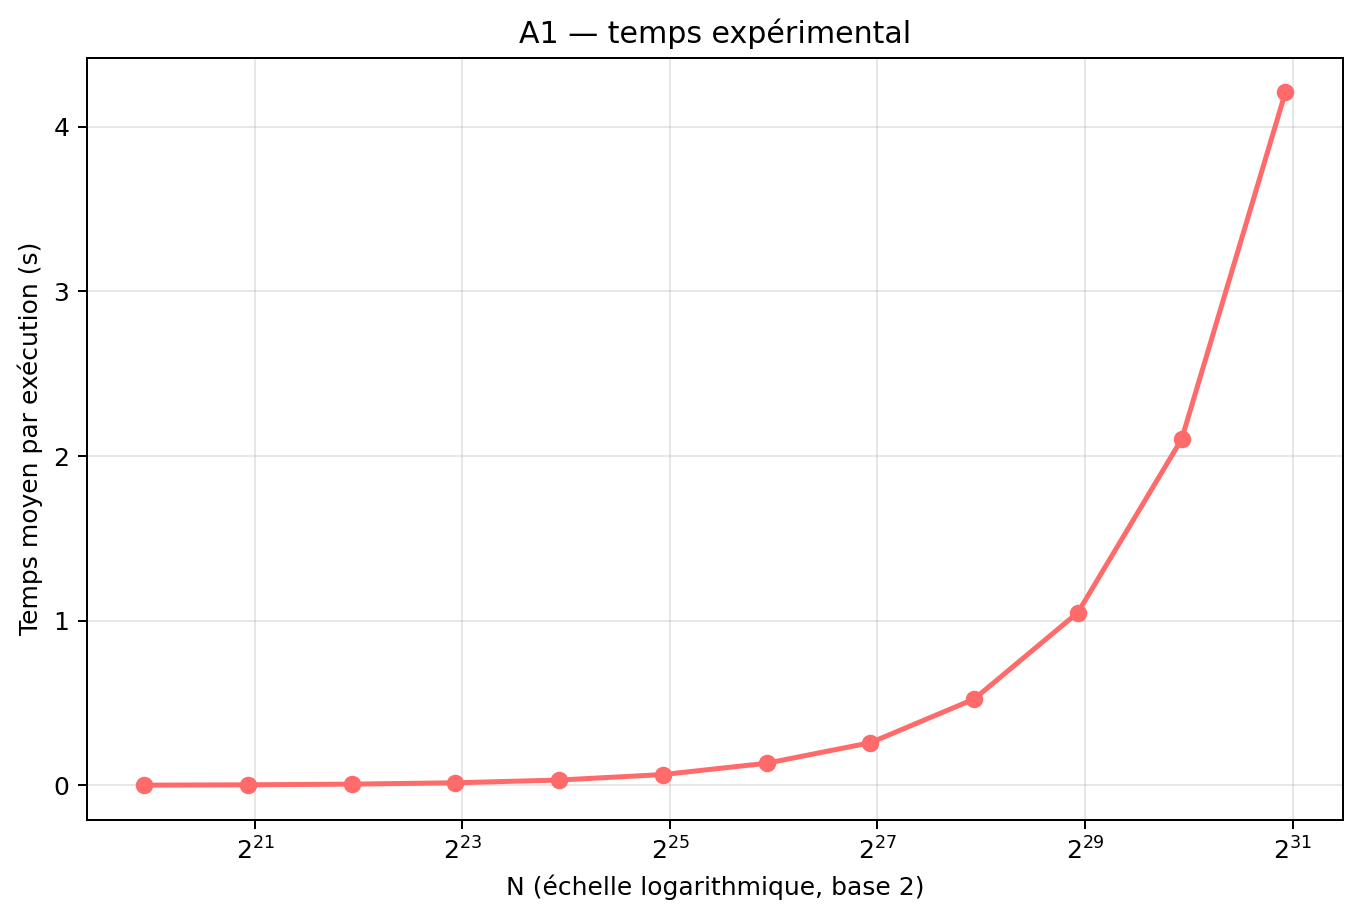
\includegraphics[width=\linewidth]{experimental_A1.png}\\
\small Temps expérimental
\end{minipage}\hfill
\begin{minipage}{0.48\textwidth}\centering
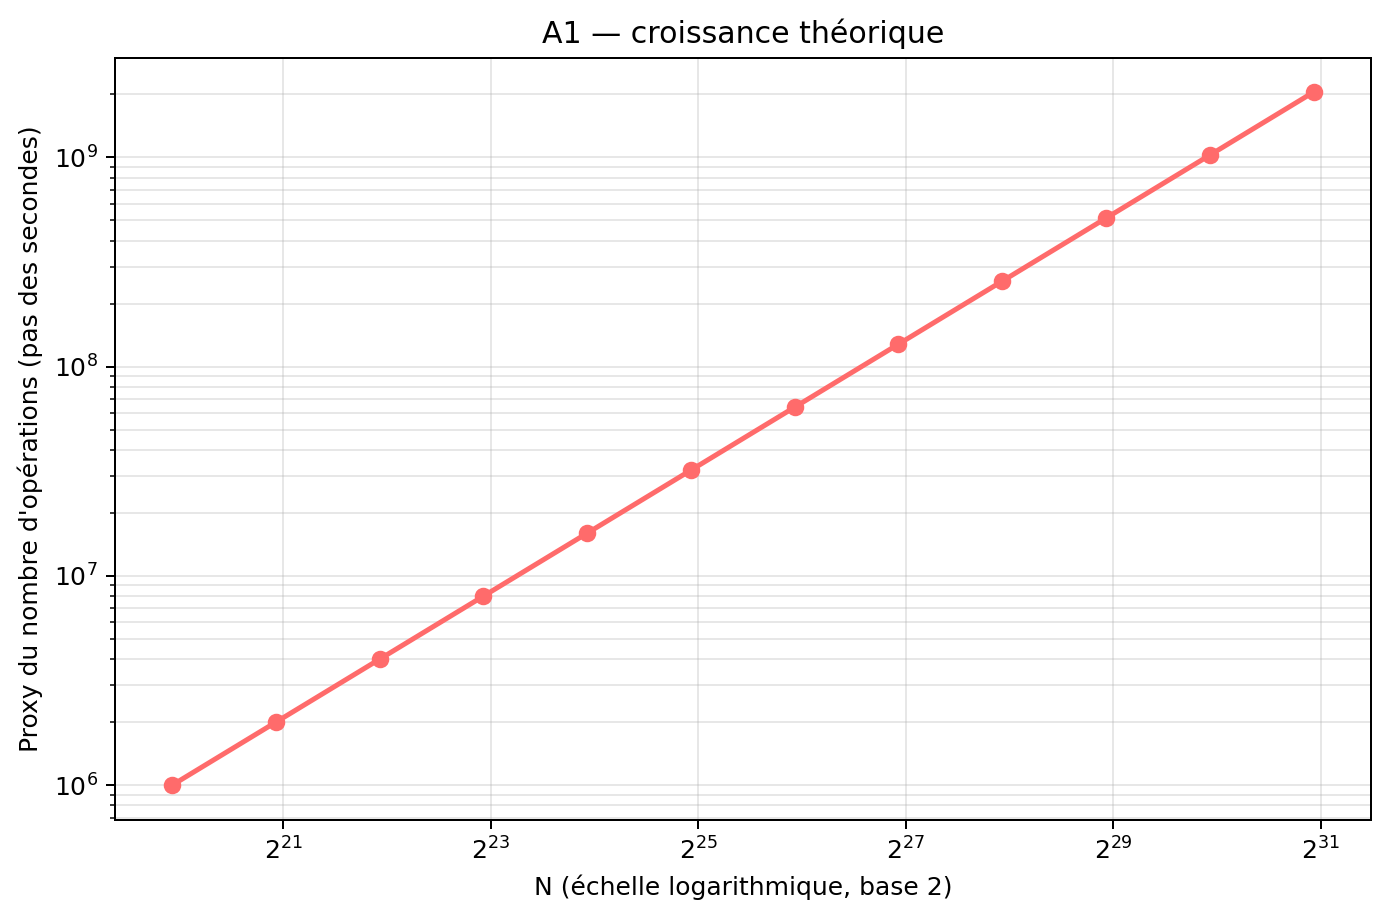
\includegraphics[width=\linewidth]{theoretical_A1.png}\\
\small Proxy théorique $N-2$
\end{minipage}
\caption{Résultats expérimentaux et croissance théorique de A1.}
\end{figure}

\subsection{A2}
\begin{figure}[H]
\centering
\begin{minipage}{0.48\textwidth}\centering
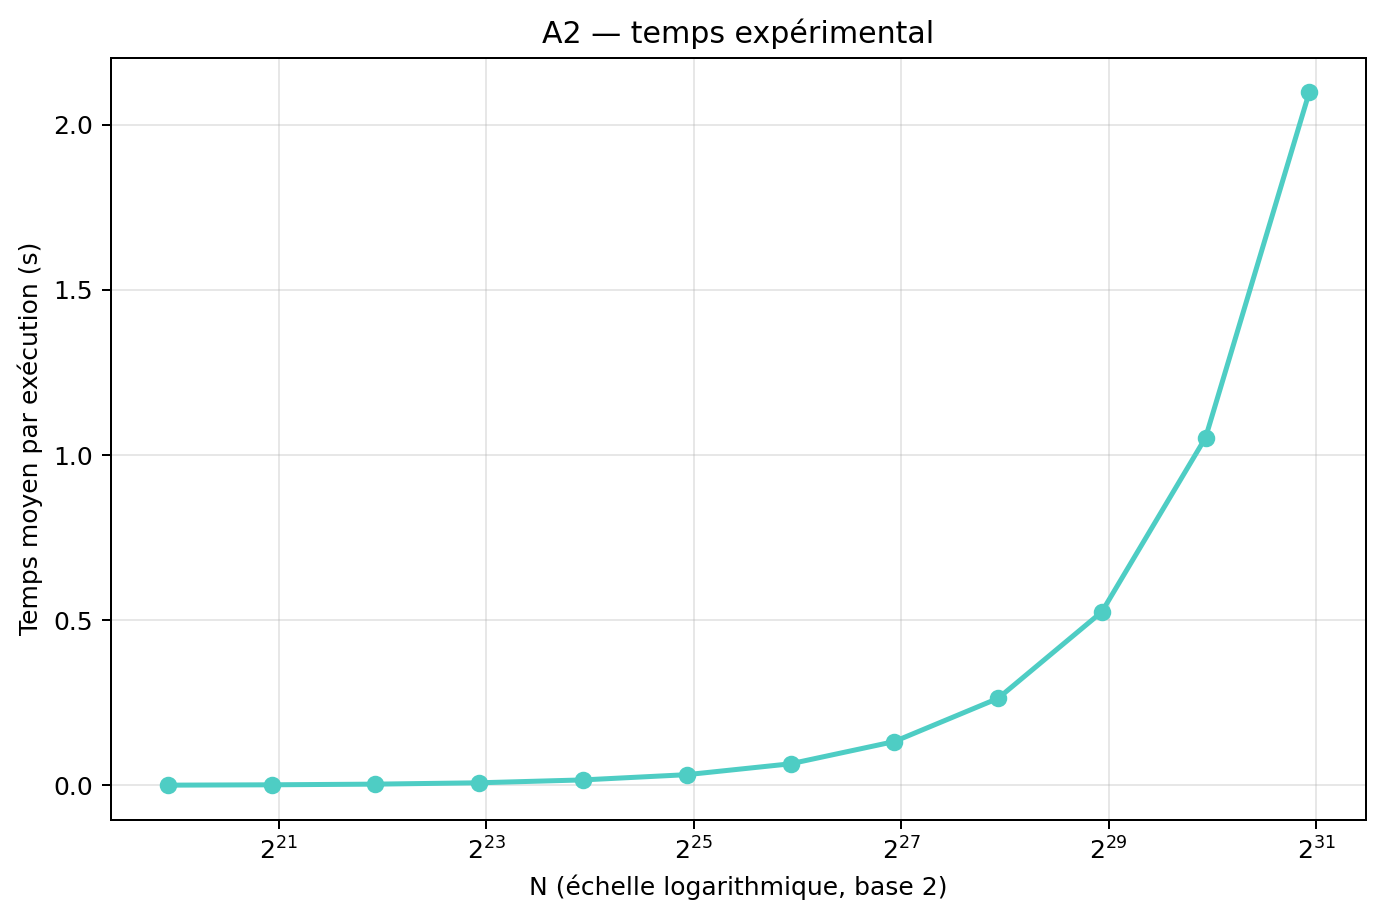
\includegraphics[width=\linewidth]{experimental_A2.png}\\
\small Temps expérimental
\end{minipage}\hfill
\begin{minipage}{0.48\textwidth}\centering
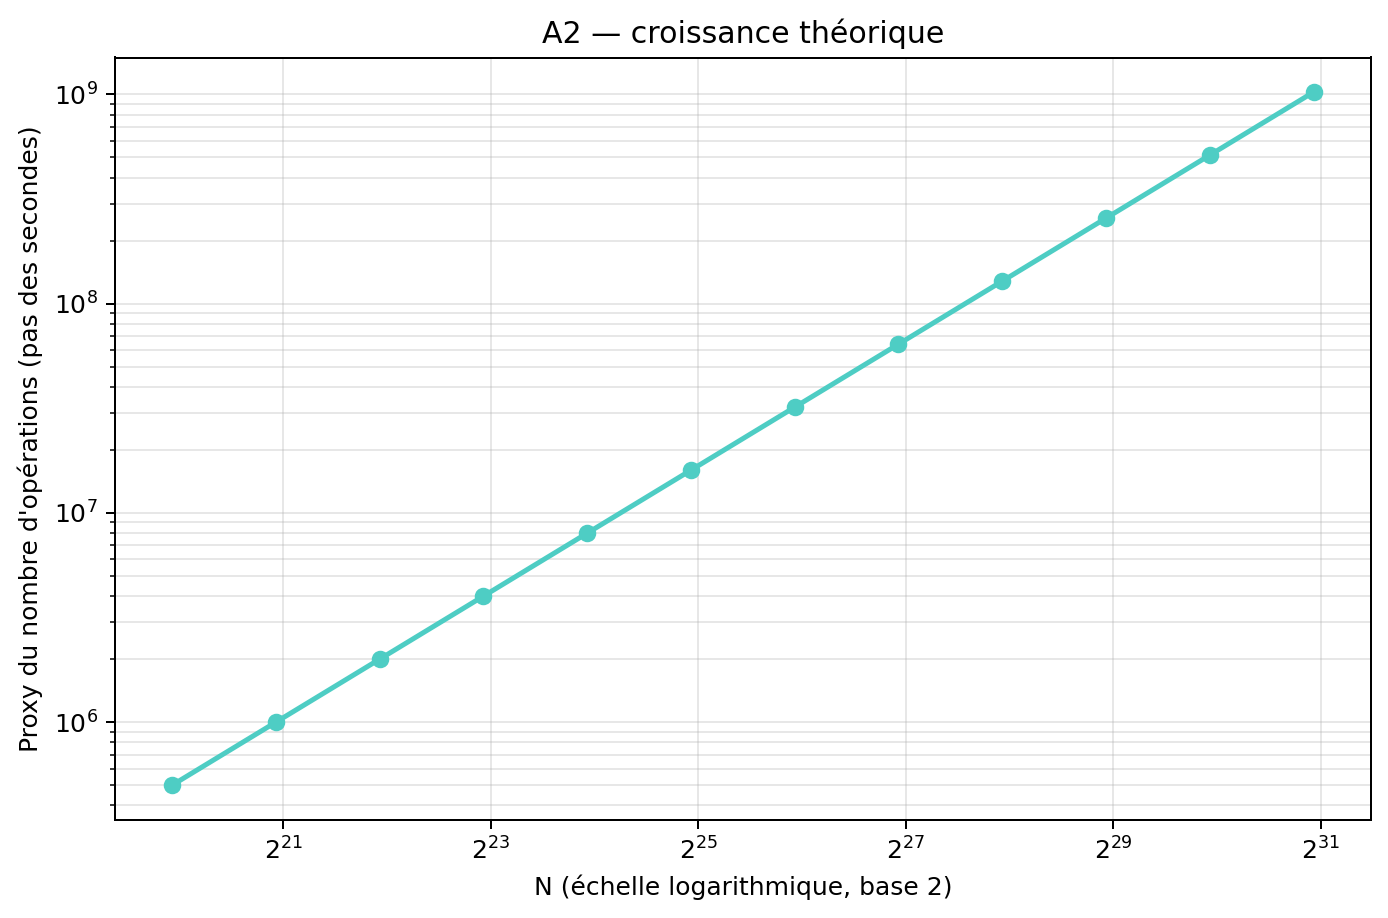
\includegraphics[width=\linewidth]{theoretical_A2.png}\\
\small Proxy théorique $N/2-1$
\end{minipage}
\caption{Résultats expérimentaux et croissance théorique de A2.}
\end{figure}

\subsection{A3}
\begin{figure}[H]
\centering
\begin{minipage}{0.48\textwidth}\centering
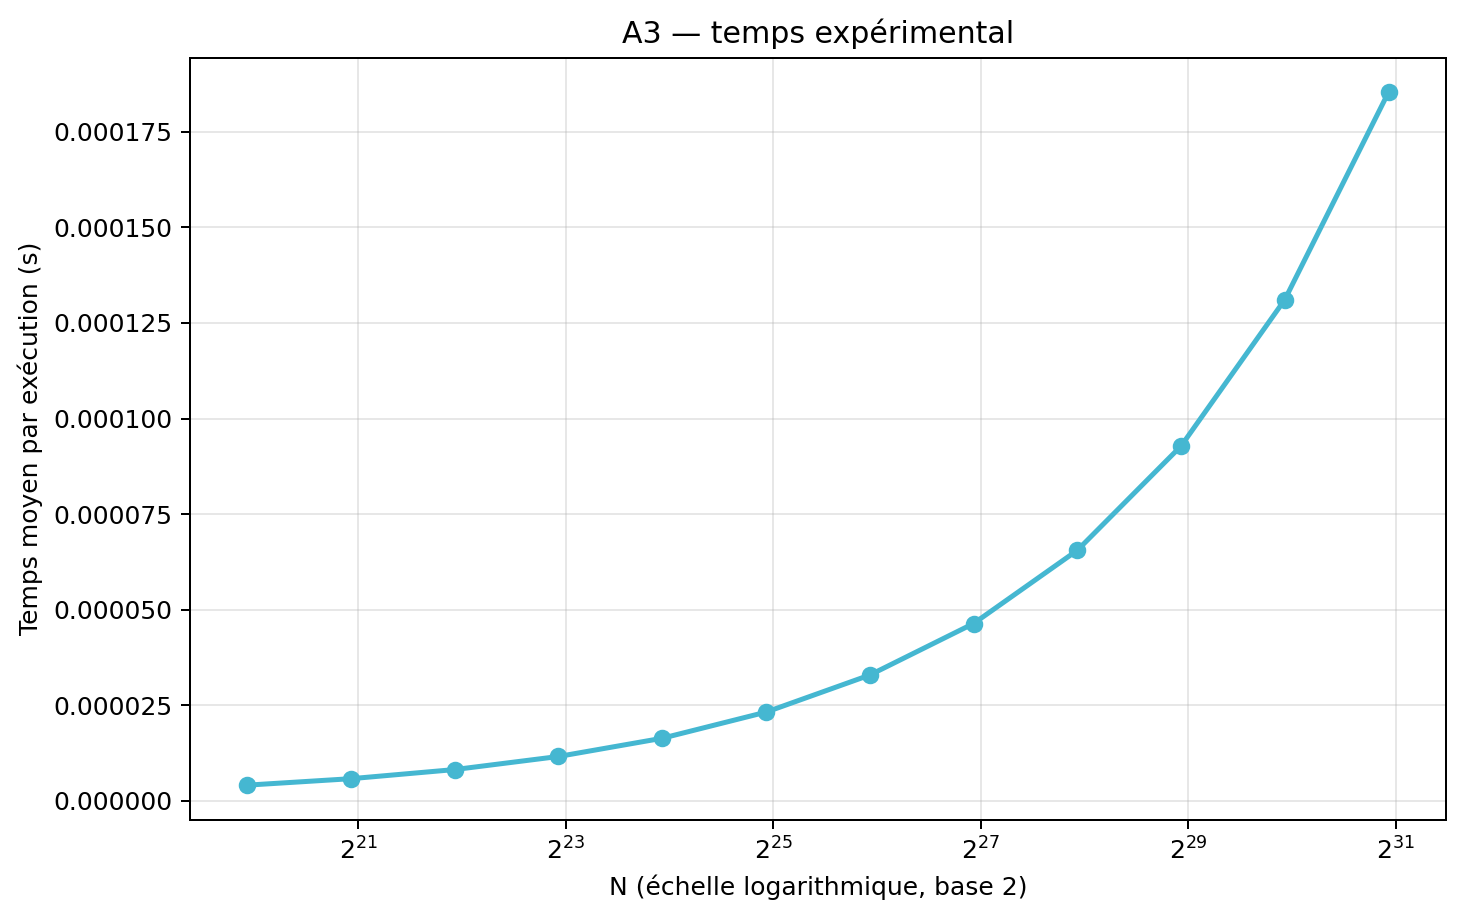
\includegraphics[width=\linewidth]{experimental_A3.png}\\
\small Temps expérimental
\end{minipage}\hfill
\begin{minipage}{0.48\textwidth}\centering
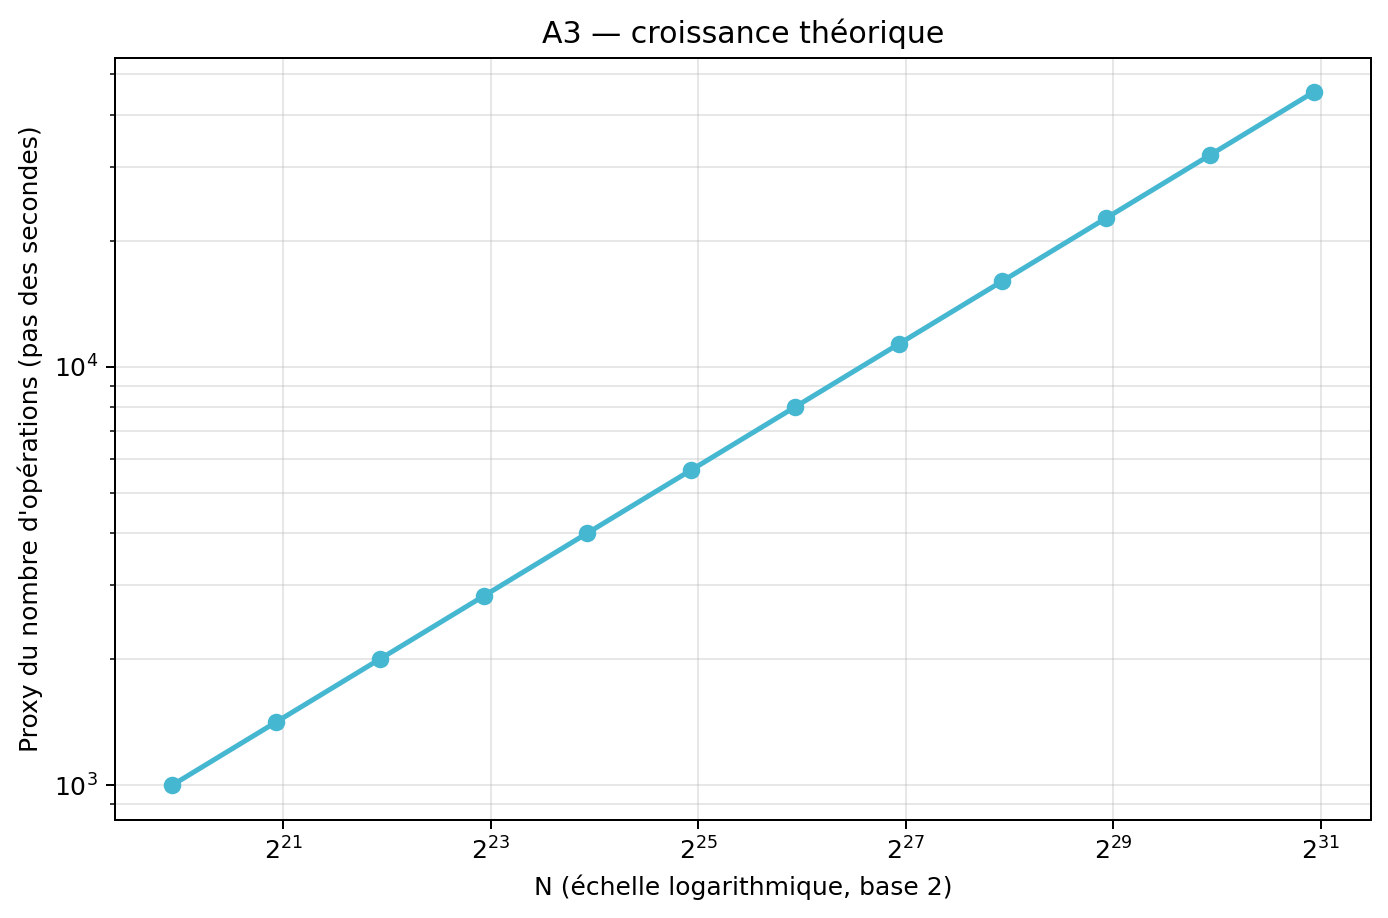
\includegraphics[width=\linewidth]{theoretical_A3.png}\\
\small Proxy théorique $\sqrt{N}$
\end{minipage}
\caption{Résultats expérimentaux et croissance théorique de A3.}
\end{figure}

\subsection{A4}
\begin{figure}[H]
\centering
\begin{minipage}{0.48\textwidth}\centering
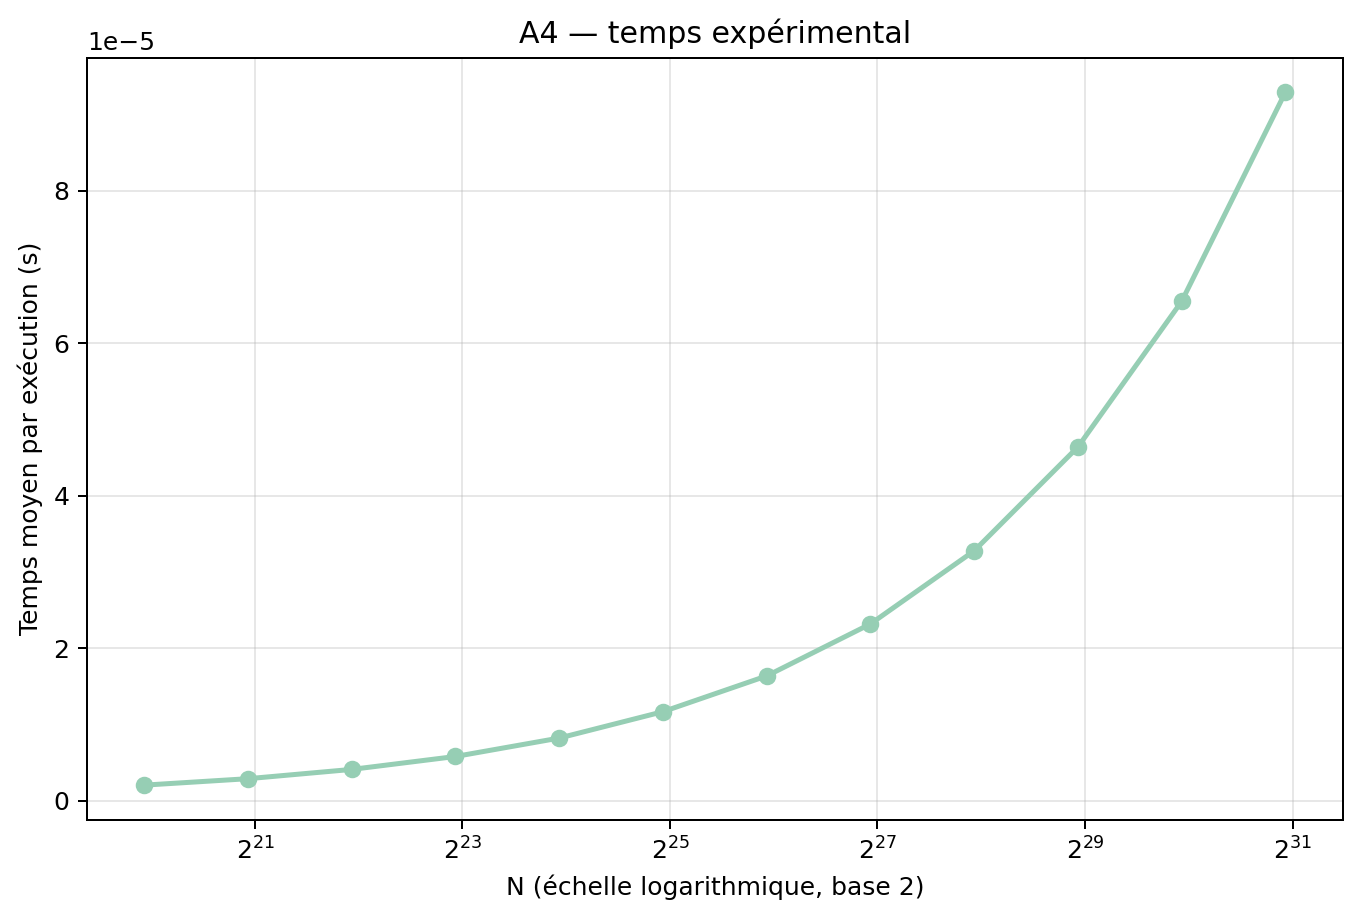
\includegraphics[width=\linewidth]{experimental_A4.png}\\
\small Temps expérimental
\end{minipage}\hfill
\begin{minipage}{0.48\textwidth}\centering
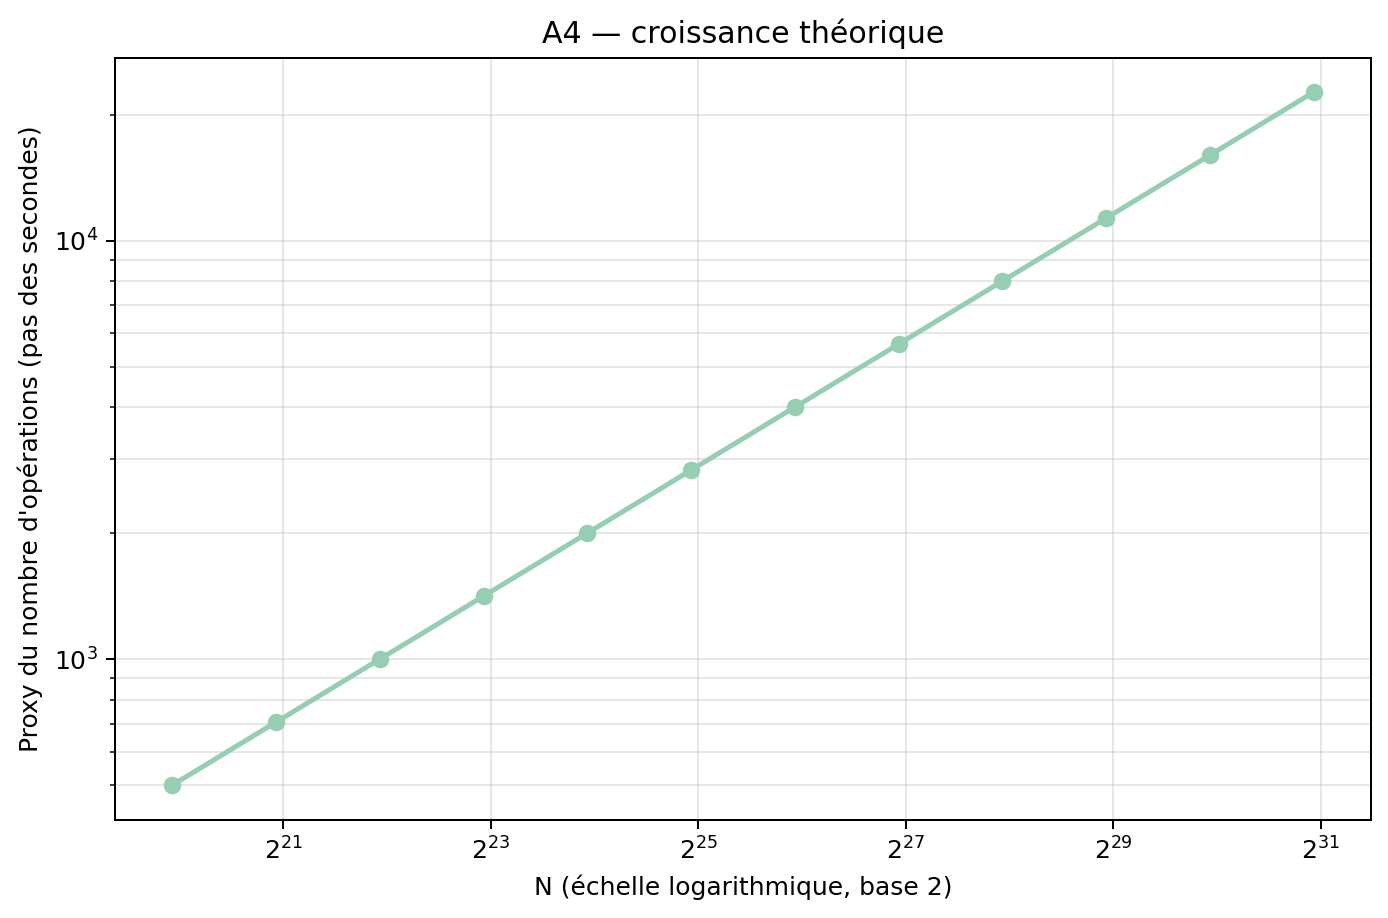
\includegraphics[width=\linewidth]{theoretical_A4.png}\\
\small Proxy théorique $\sqrt{N}/2$
\end{minipage}
\caption{Résultats expérimentaux et croissance théorique de A4.}
\end{figure}

\subsection{Comparaisons progressives}

\begin{figure}[H]
\centering
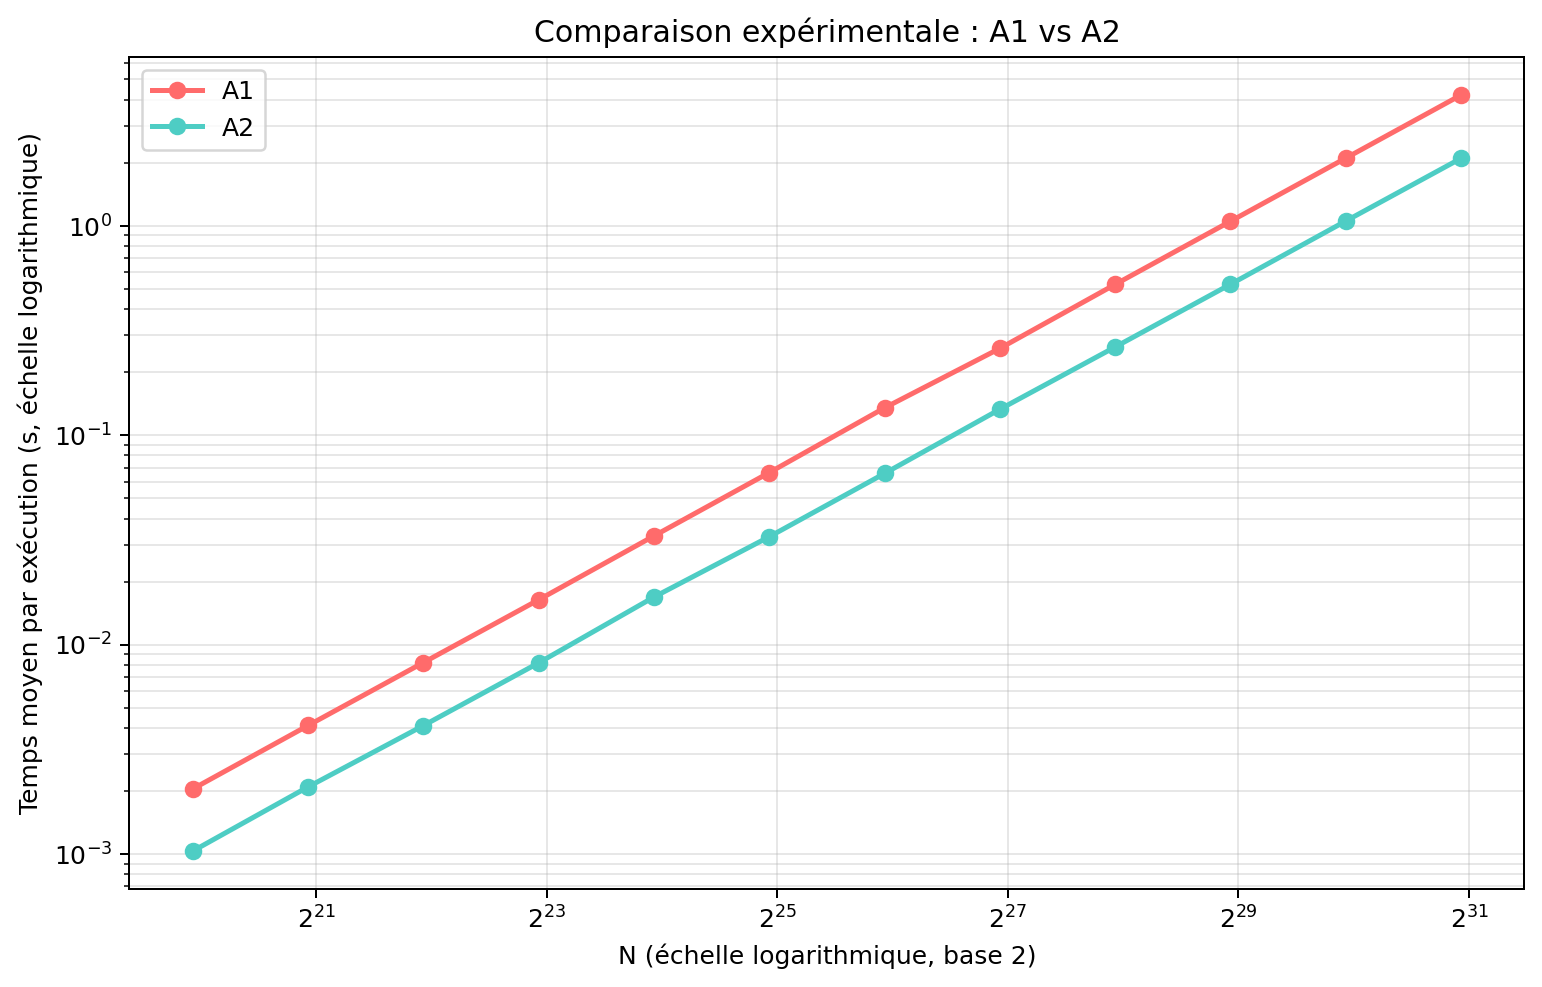
\includegraphics[width=0.92\textwidth]{comparison_A1_A2.png}
\caption{Comparaison expérimentale de A1 et A2.}
\end{figure}

\begin{figure}[H]
\centering
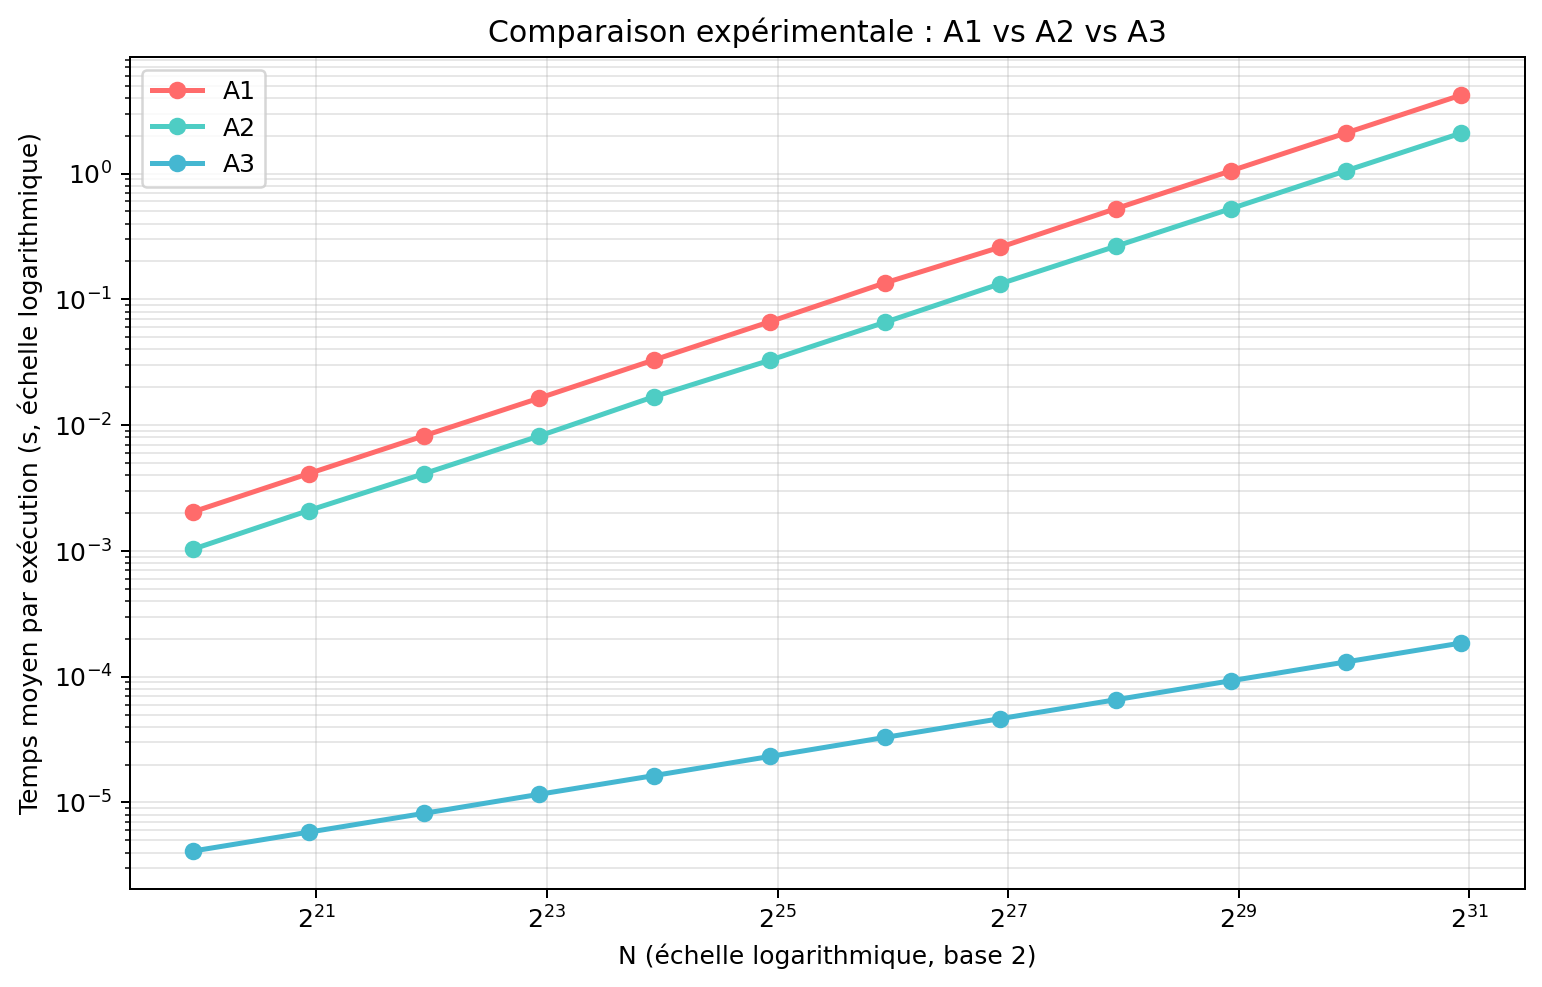
\includegraphics[width=0.92\textwidth]{comparison_A1_A2_A3.png}
\caption{Comparaison expérimentale de A1, A2 et A3.}
\end{figure}

\begin{figure}[H]
\centering
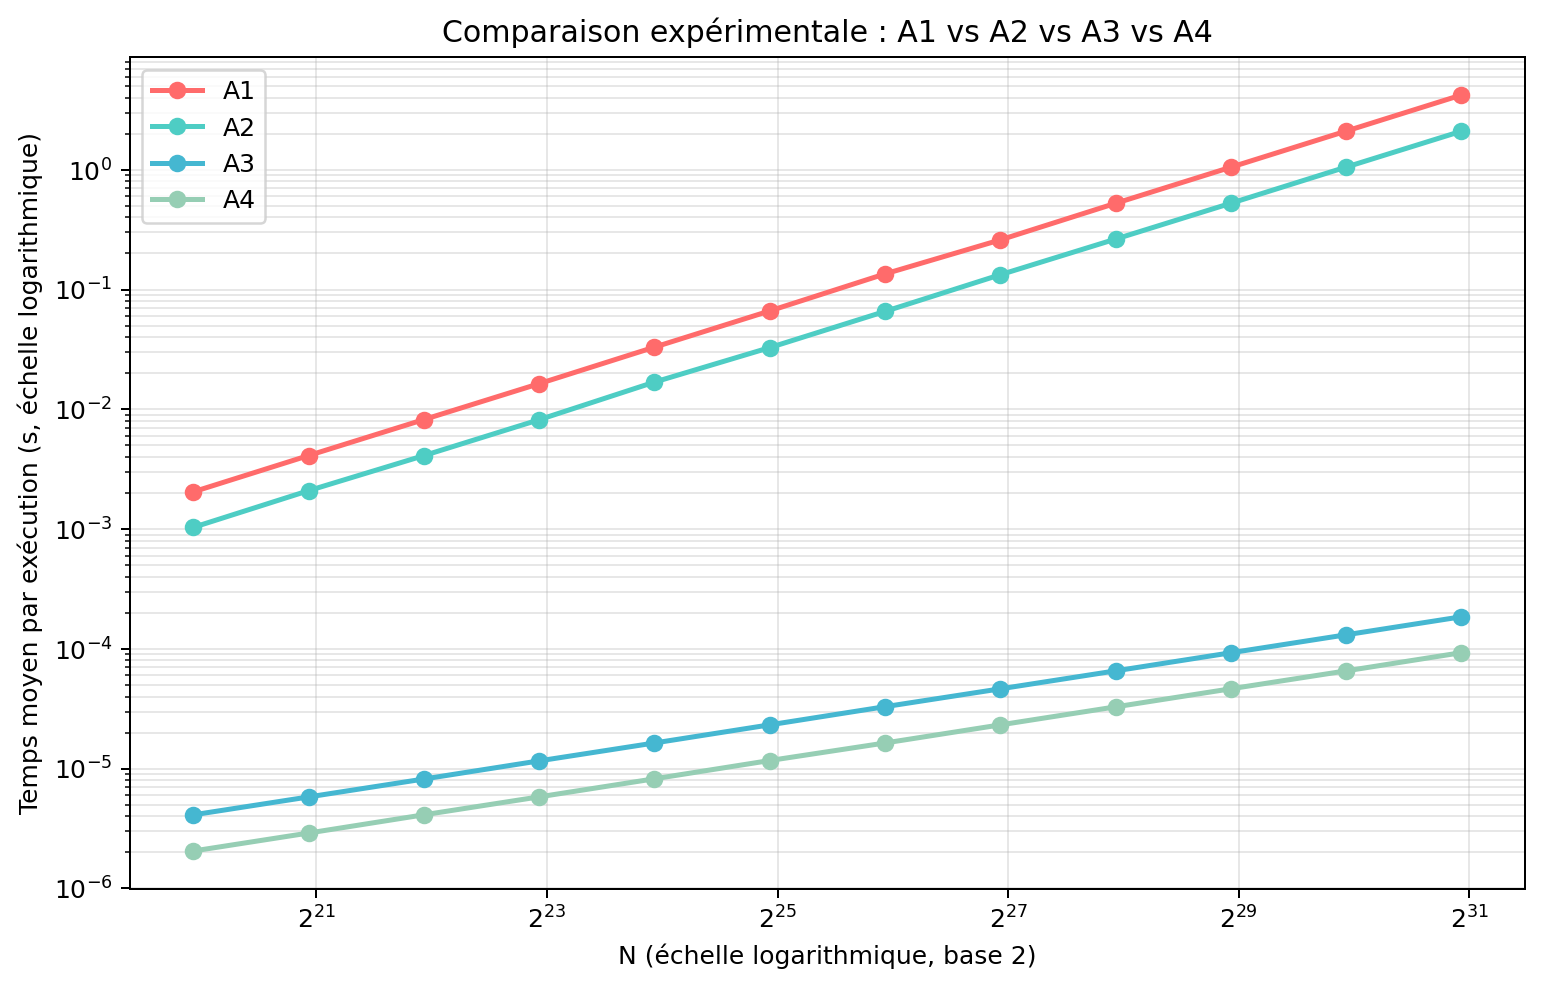
\includegraphics[width=0.92\textwidth]{comparison_A1_A2_A3_A4.png}
\caption{Comparaison expérimentale des quatre algorithmes.}
\end{figure}

\subsection{Graphiques des cinq jeux de données}

Les figures suivantes comparent les temps mesurés pour les entrées de chaque jeu. Les points \texttt{SKIP} ne sont pas tracés.

\begin{figure}[H]
\centering
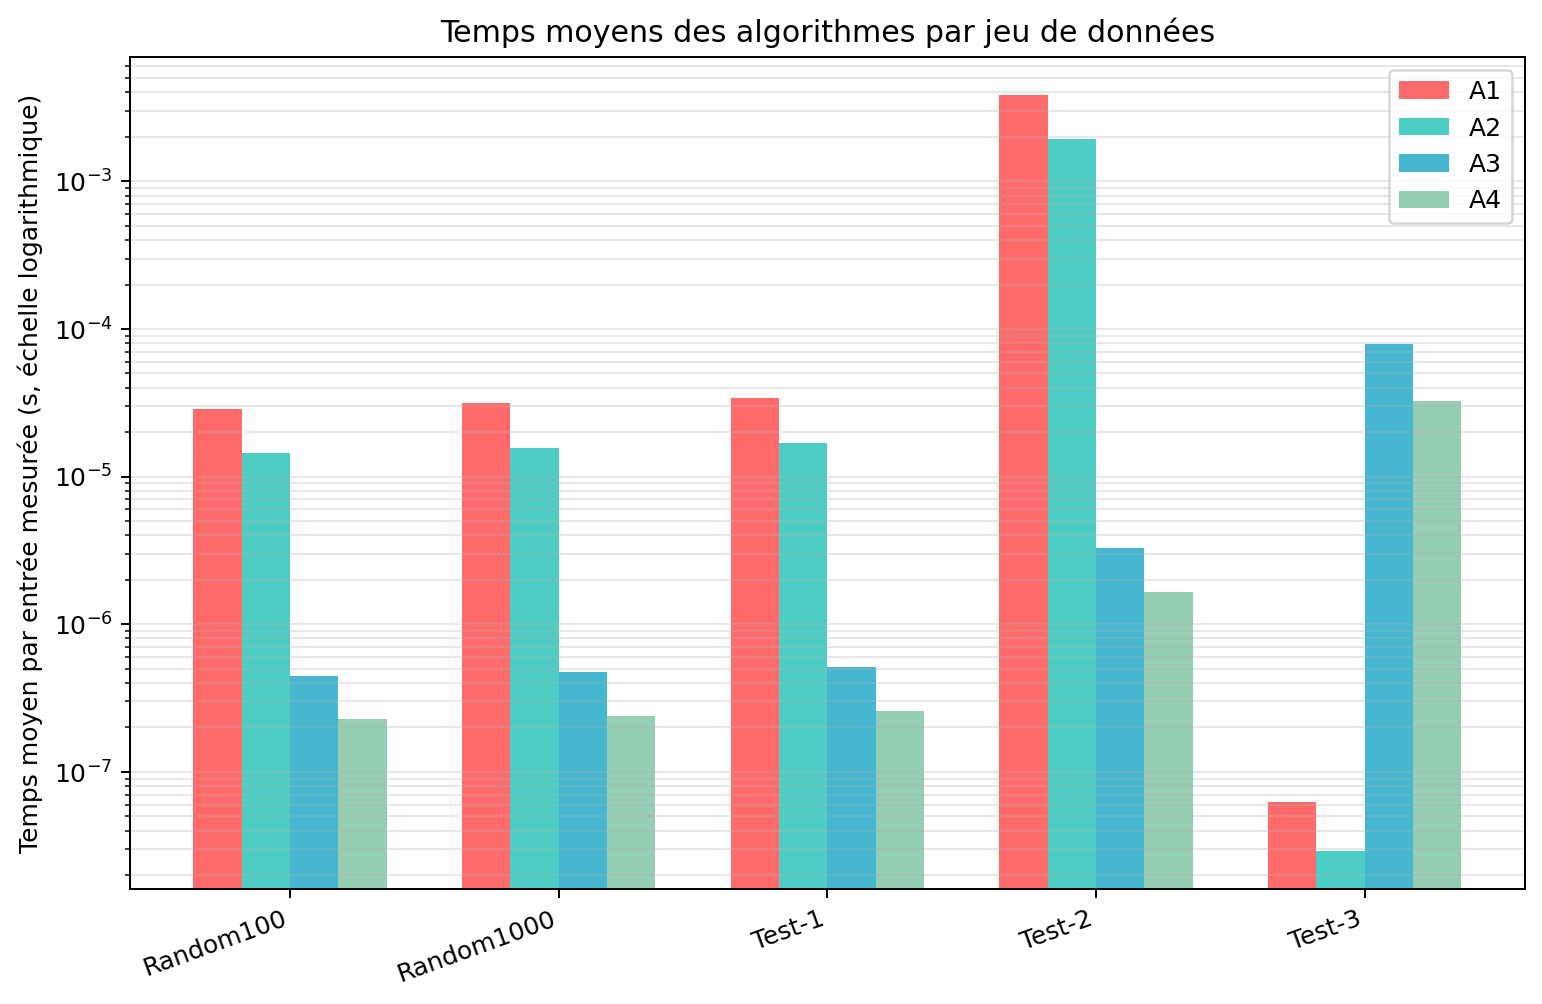
\includegraphics[width=0.88\textwidth]{datasets_comparison.png}
\caption{Temps moyens par entrée mesurée, regroupés par jeu de données.}
\end{figure}

\begin{figure}[H]
\centering
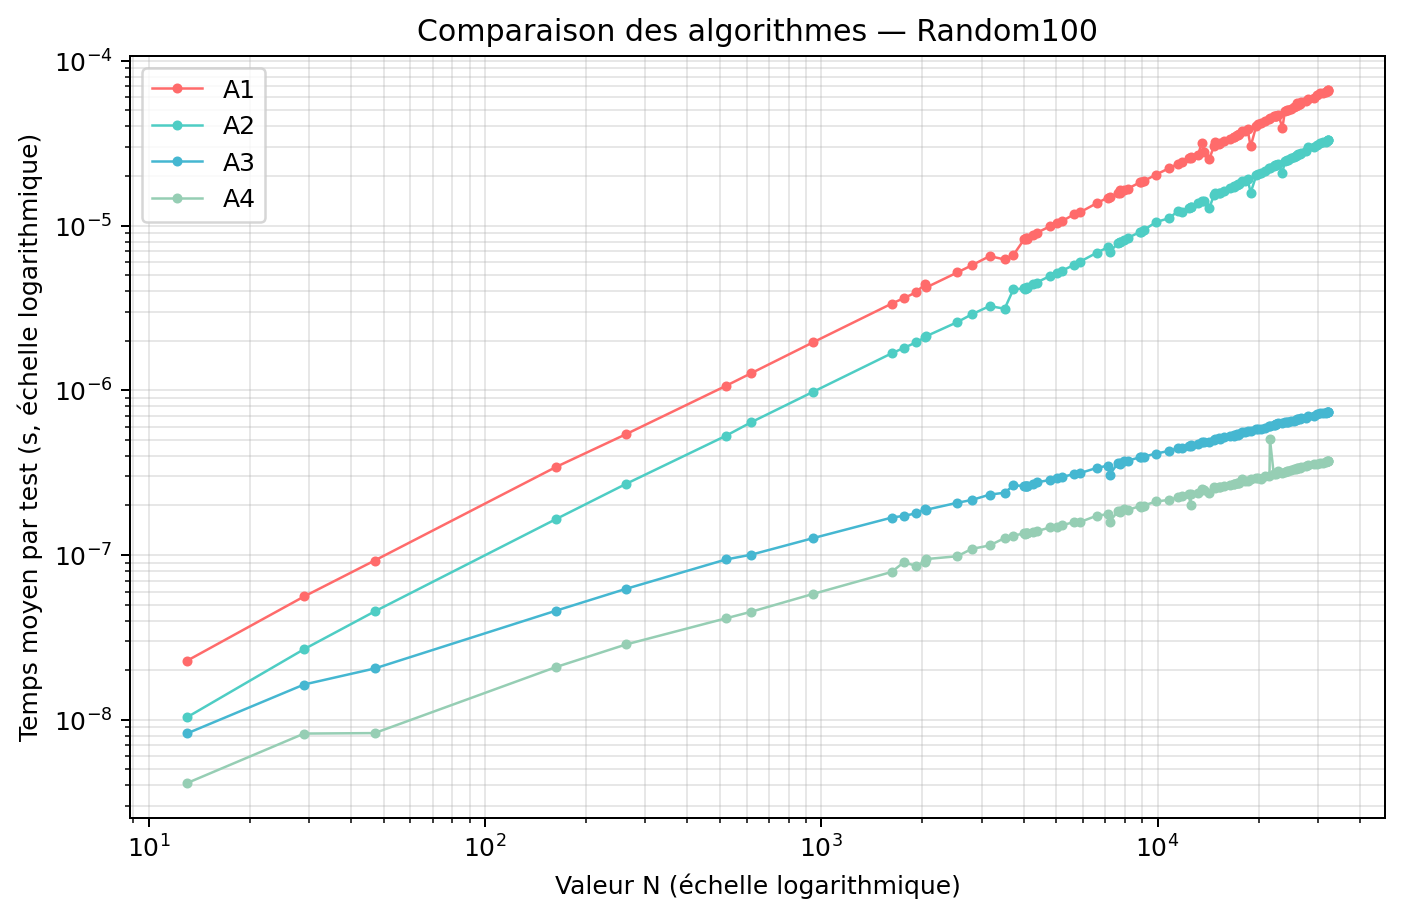
\includegraphics[width=0.88\textwidth]{datasets_Random100.png}
\caption{Comparaison des algorithmes sur Random100.}
\end{figure}

\begin{figure}[H]
\centering
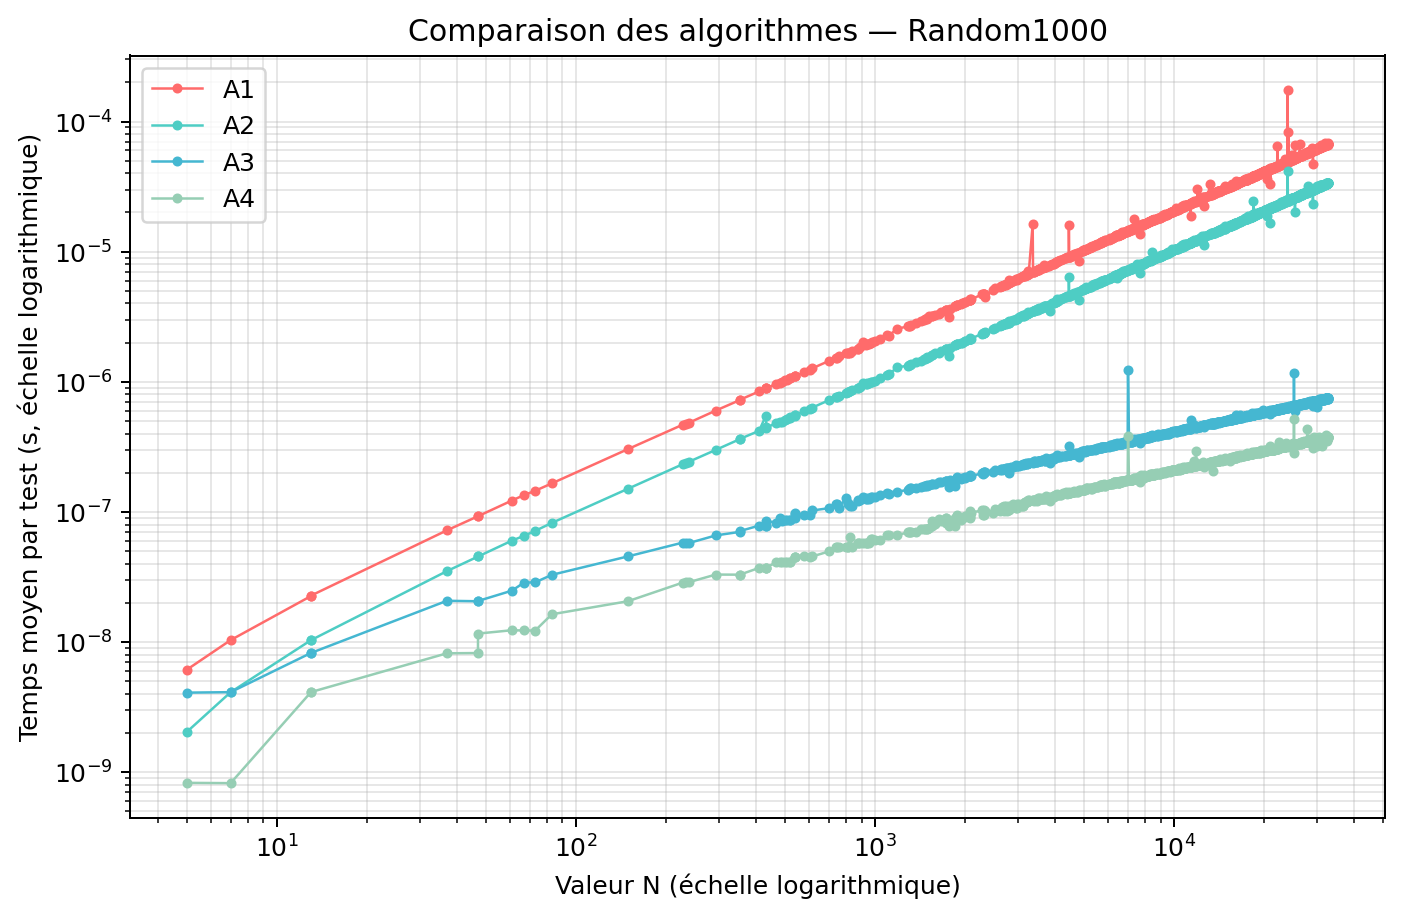
\includegraphics[width=0.88\textwidth]{datasets_Random1000.png}
\caption{Comparaison des algorithmes sur Random1000.}
\end{figure}

\begin{figure}[H]
\centering
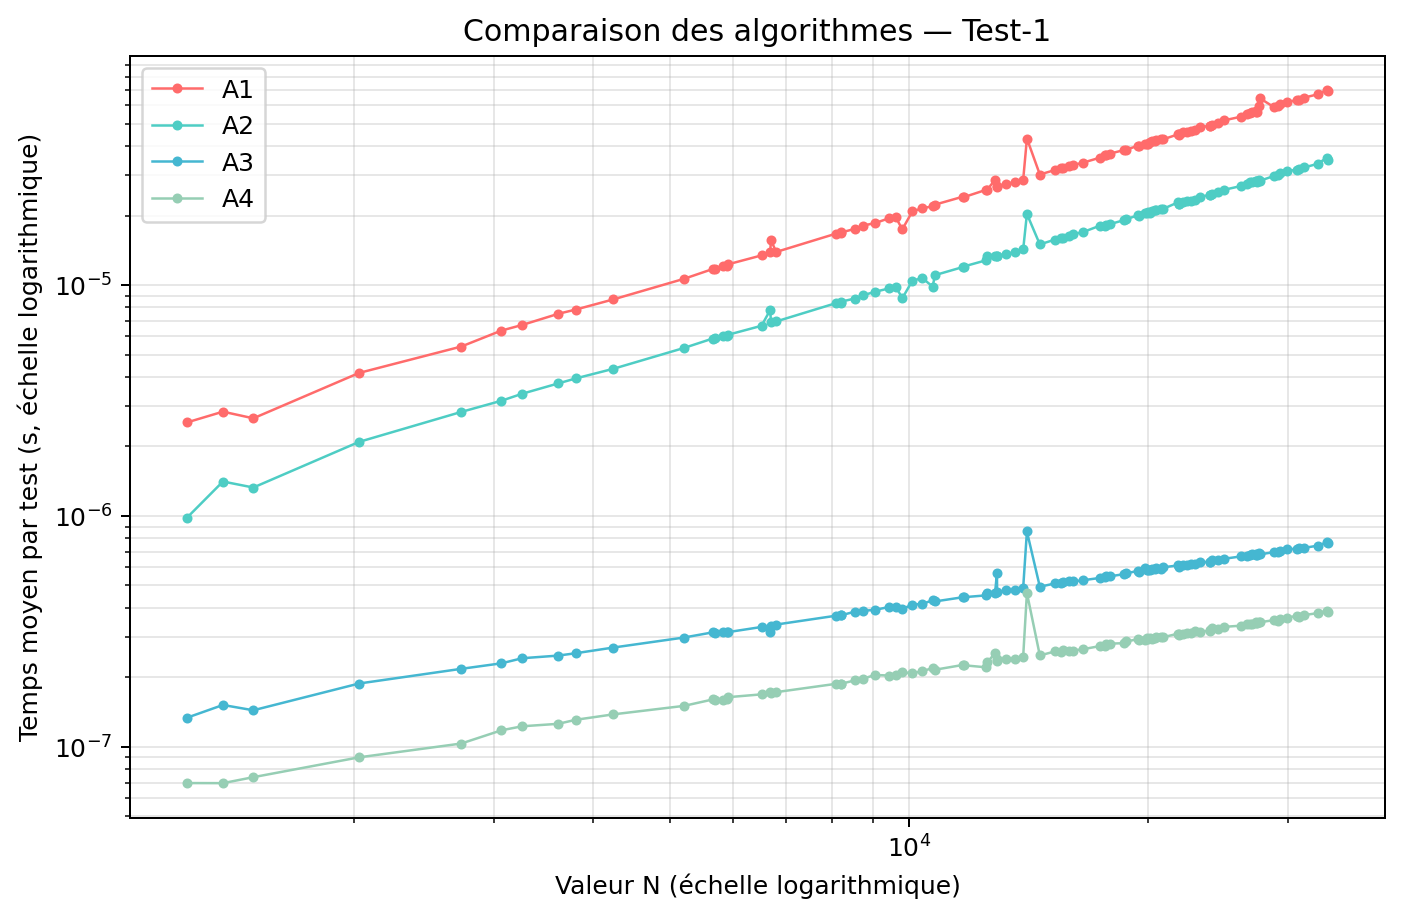
\includegraphics[width=0.88\textwidth]{datasets_Test-1.png}
\caption{Comparaison des algorithmes sur Test-1.}
\end{figure}

\begin{figure}[H]
\centering
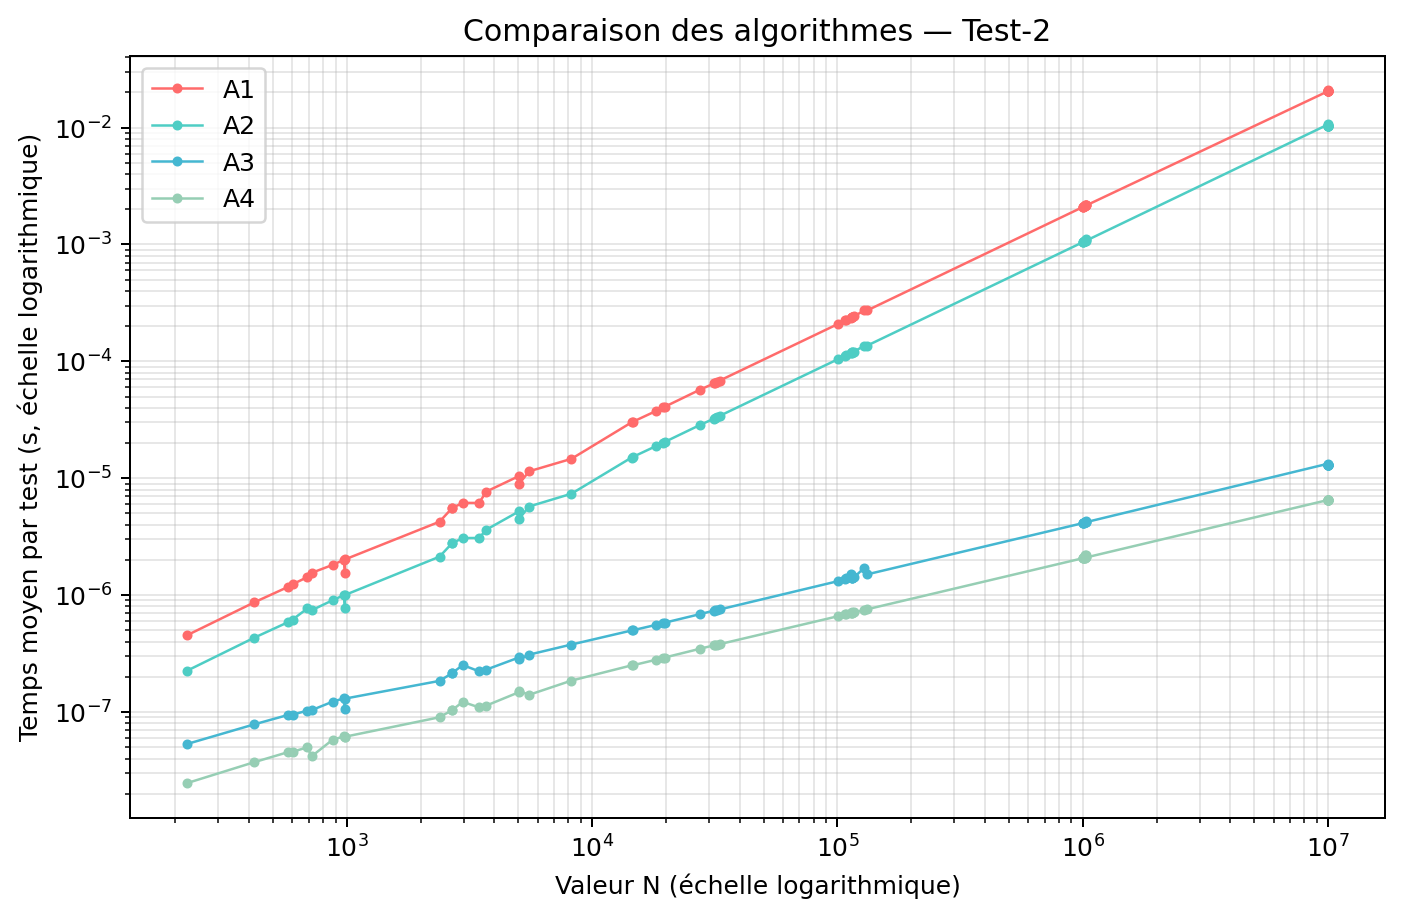
\includegraphics[width=0.88\textwidth]{datasets_Test-2.png}
\caption{Comparaison des algorithmes sur Test-2.}
\end{figure}

\begin{figure}[H]
\centering
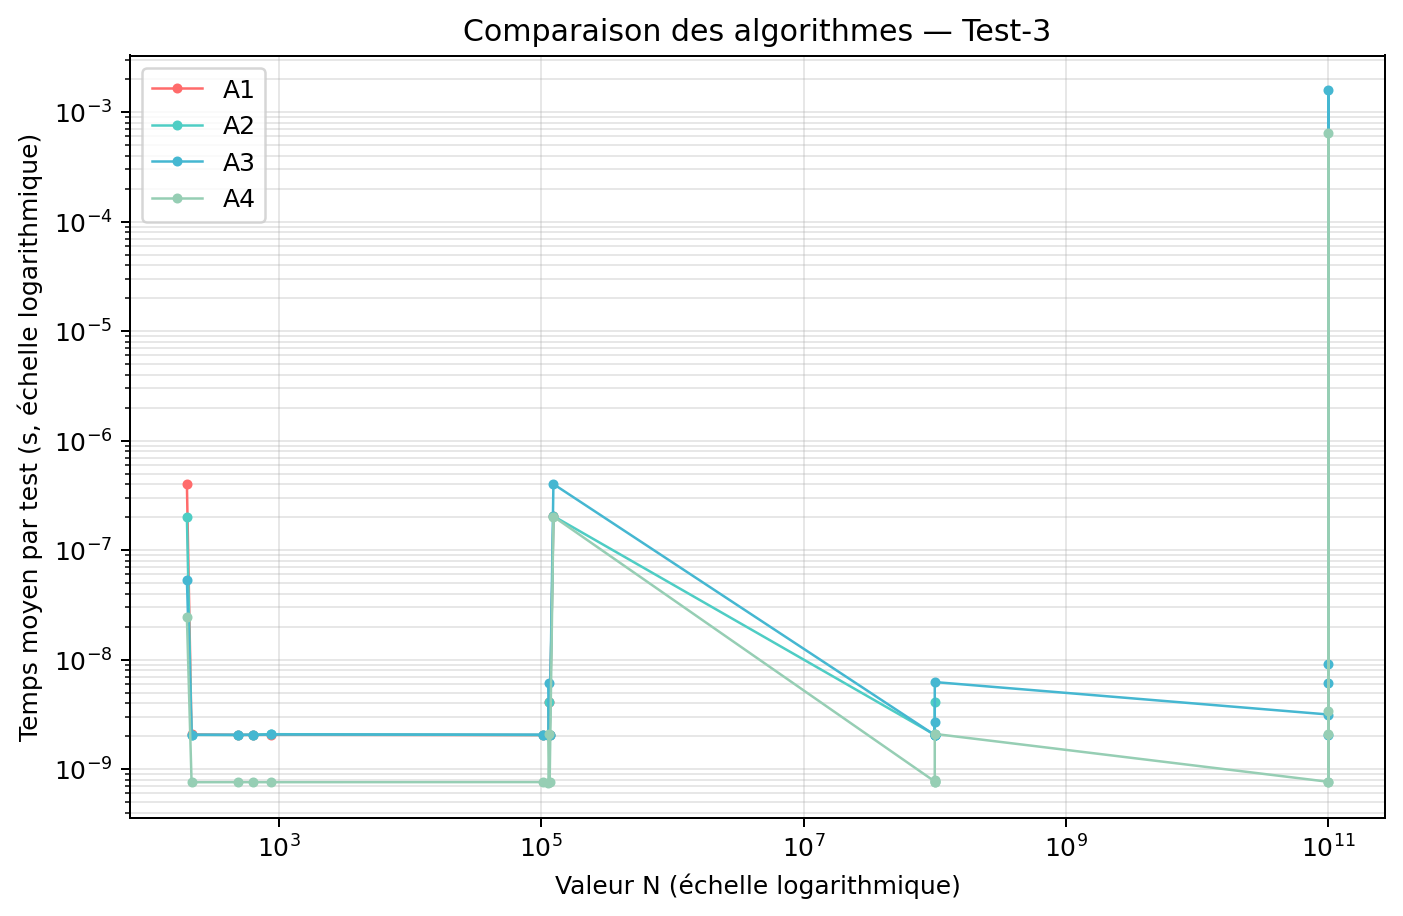
\includegraphics[width=0.88\textwidth]{datasets_Test-3.png}
\caption{Comparaison des algorithmes sur Test-3.}
\end{figure}

\section{Conclusion}

Les mesures des douze valeurs du sujet et des cinq jeux de données confirment l'intérêt des améliorations successives. A2 réduit le temps par un facteur constant sans changer la complexité linéaire. A3 obtient une amélioration asymptotique en limitant les tests à $\sqrt{N}$. A4 conserve cette complexité et réduit encore le travail sur les entrées impaires en ignorant les diviseurs pairs. Les résultats détaillés indiquent aussi les valeurs écartées pour A1 et A2 dans Test-3 en raison de leur coût excessif.

\end{document}
